\chapter{Results}

\section{Fiducial WZjj cross section measurement}

The cross section for \WZjj production, without separating by production mechanism,
is measured with a combined maximum likelihood fit to the 
observed event yields.
The likelihood is a combination of individual likelihoods for the four decay channels for the
signal and background hypotheses with the statistical and systematic uncertainties in the form
of nuisance parameters. 
The expected event yields for the EW- and QCD-induced \WZjj processes
are taken from the \MG~v2.4.2 predictions. 
A signal strength $\mu_{\WZjj}$, which represents the 
ratio of the measured signal yield to the expected number of signal events, 
is treated as a free parameter in the fit.

\begin{figure}[htbp]
  \centering
   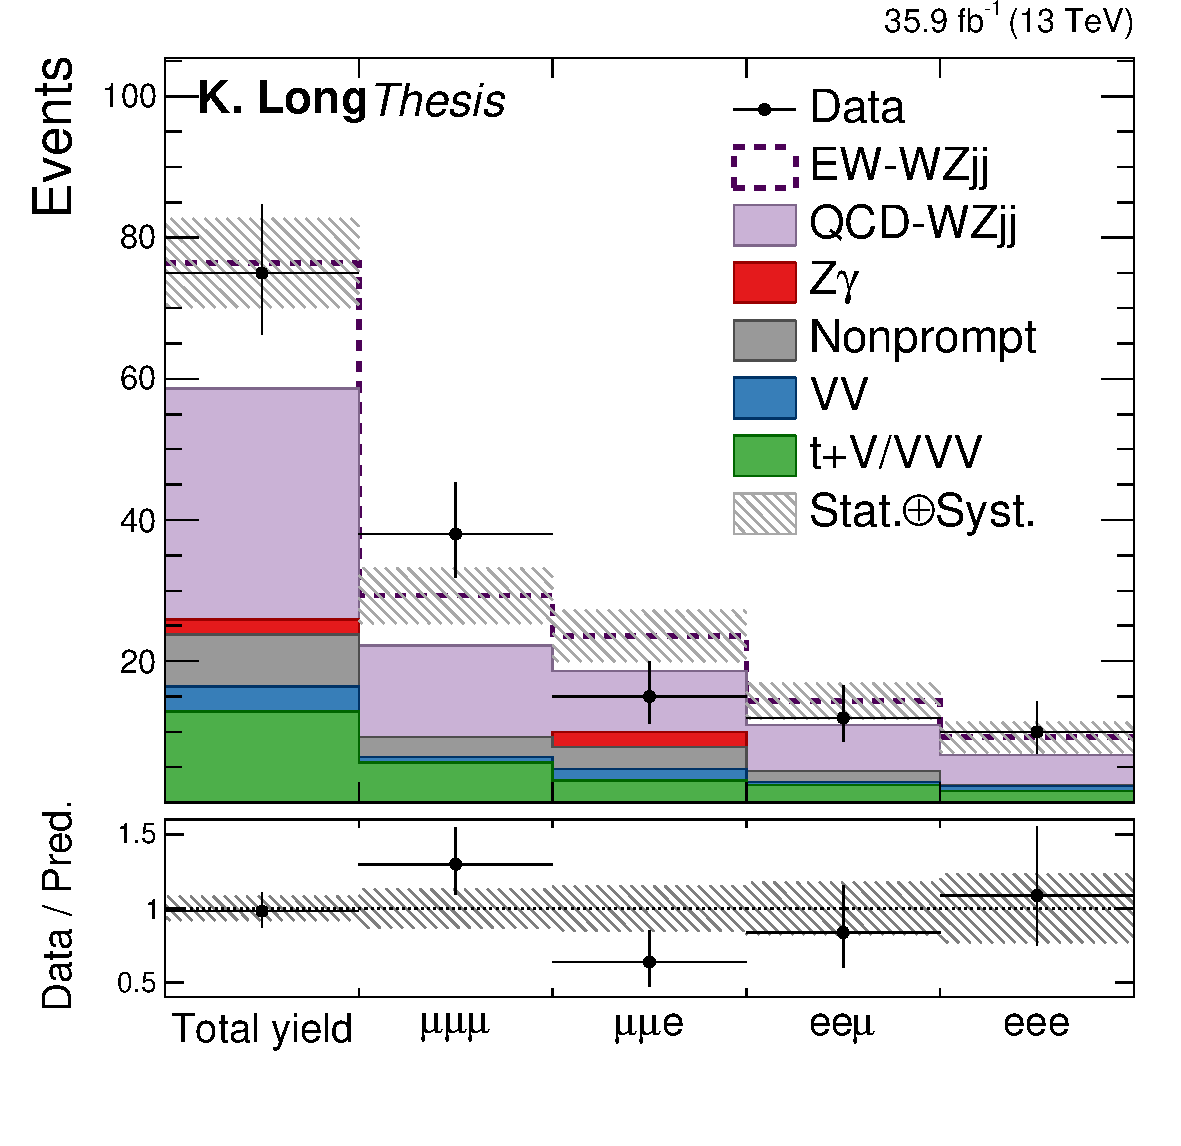
\includegraphics[width=0.7\textwidth]{figures/AnalysisResults/yieldByChannel.pdf}
  \caption{
    Post fit event yields in the EW signal region.
          }
 \label{fig:EWSignalYields}
\end{figure}

The best fit value for the signal strength is used to obtain a cross section
in the tight fiducial region defined in Table~\ref{tab:selections}. 
The measured fiducial \WZjj cross section in this region is

\begin{equation}
  \sigma^{\mathrm{fid}}_{\mathrm{WZjj}} = 
        3.18^{+0.57}_{-0.52} \, \mathrm{(stat)} \,\, ^{+0.43}_{-0.36} \, \mathrm{(syst)}
        = 3.18^{+0.71}_{-0.63} \,\unit{fb} \,.
\end{equation}

This result can be compared to the predicted value of
$3.27 \, ^{+0.39}_{-0.32} \mathrm{(scale)} \pm 0.15\, \mathrm{(PDF)} \unit{fb}$.
The \EWWZ and \QCDWZ contributions are
calculated independently from the samples described in Section~\ref{sec:mc}
and their uncertainties are combined in quadrature. 
The interference term contribution in this region is less than 1\% of
the total cross section.

Results are also obtained in a looser fiducial region, defined in Table~\ref{tab:selections}
following Ref.~\cite{leshouches2017},
to simplify comparisons with theoretical calculations.
The acceptance from the loose to tight fiducial region
is $(72.4 \pm 0.8)\%$,
computed using \MG interfaced to \PYTHIA. 
The uncertainty in the acceptance is evaluated independently 
for the \EWWZ and \QCDWZ samples
from the scale
and PDF uncertainties, which are combined in quadrature.
The scale uncertainty in the \QCDWZ contribution is the 
dominant component of the uncertainty.
The resulting \WZjj loose fiducial cross section is

\begin{equation}
  \sigma^{\mathrm{fid, loose}}_{\mathrm{WZjj}} = 
        4.39^{+0.78}_{-0.72} \, \mathrm{(stat)} \,\, ^{+0.60}_{-0.50} \, \mathrm{(syst)}
        = 4.39^{+0.98}_{-0.87} \,\unit{fb} \,,
\end{equation}

which can be compared to the predicted value of 
$4.51^{+0.59}_{-0.45} \, \mathrm{(scale)} \pm 0.18 \, \mathrm{(PDF)} \unit{fb}$.
The \EWWZ and \QCDWZ contributions 
and their uncertainties are treated independently with the same approach as described
for the tight fiducial region.

\section{Search for EW WZ boson production}

\begin{figure}[htbp]
  \centering
   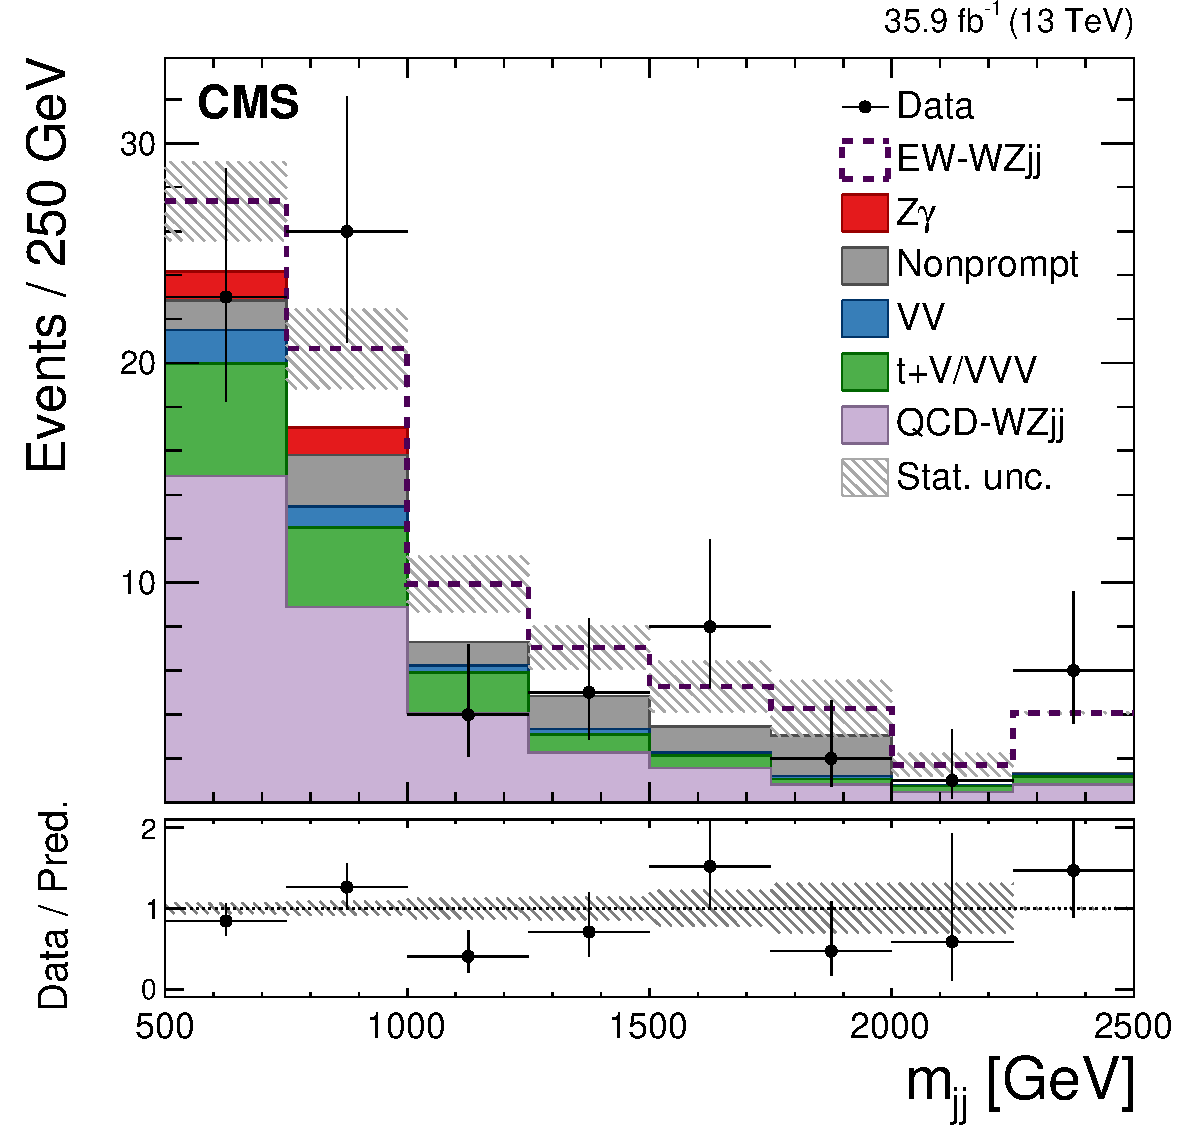
\includegraphics[width=0.7\textwidth]{figures/AnalysisResults/mjj.pdf}
   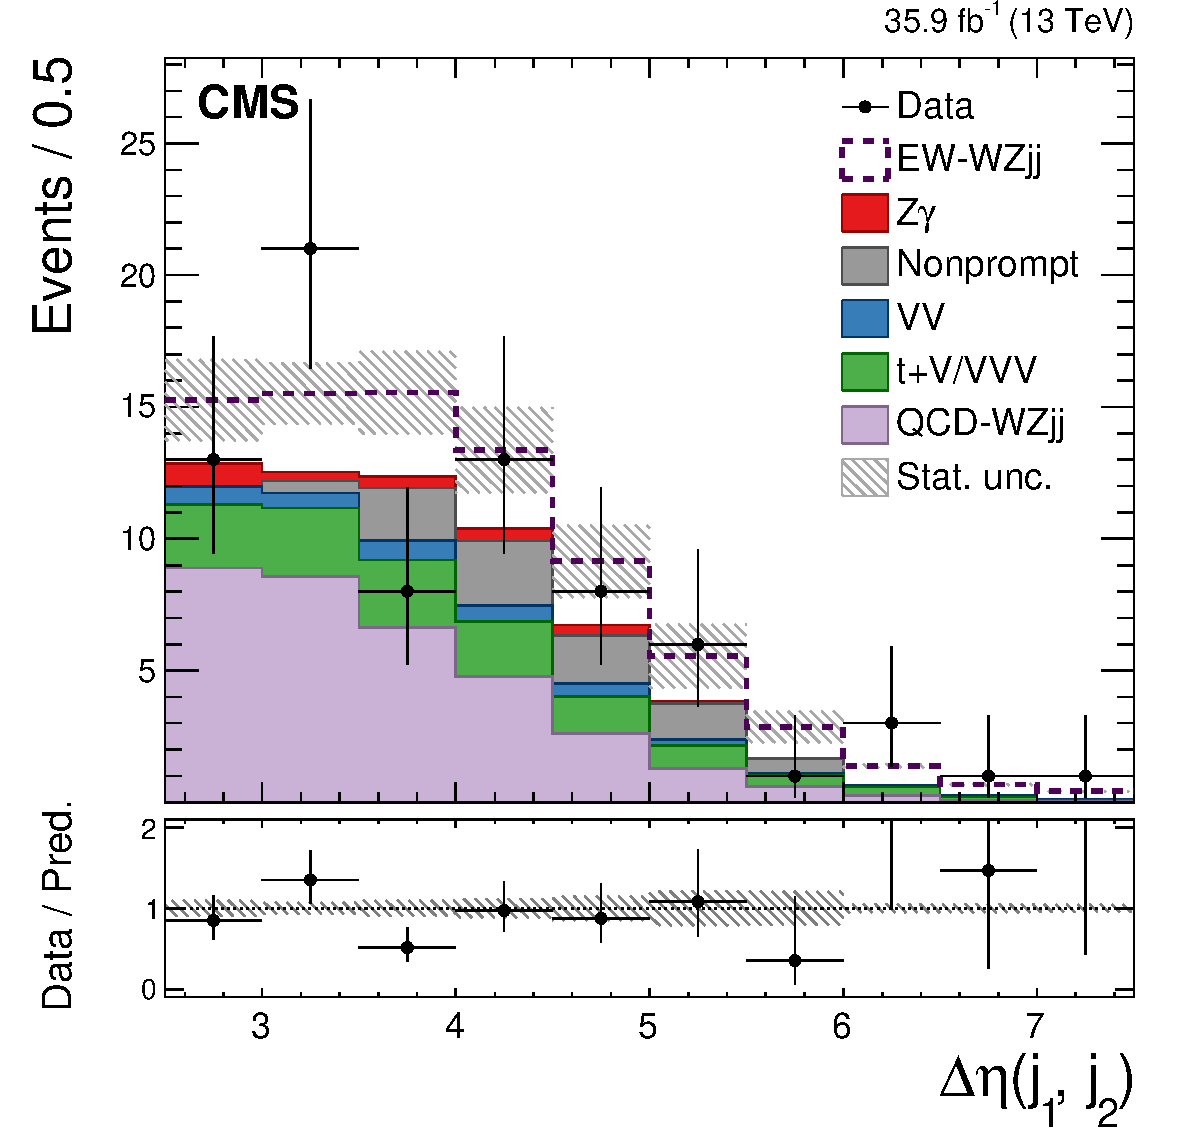
\includegraphics[width=0.7\textwidth]{figures/AnalysisResults/dEtajj.pdf}
  \caption{
  The $\mjj$ (left) and $\left|\etajj\right|$ 
  of the two leading jets 
  (right) for events satisfying the EW signal selection. 
  The last bin contains all events with $\mjj > 2500\GeV$ (left) and 
  $\left|\etajj\right| > 7.5$ (right).
  The dashed line shows the expected \EWWZ contribution stacked
  on top of the backgrounds, which are shown as filled histograms. 
  The hatched bands represent the total and relative 
  statistical uncertainties on the predicted yields.
  The bottom panel shows the ratio of the number of events measured in data to the total 
  number of expected events. 
  The predicted yields are shown with their prefit normalizations.
          }
 \label{fig:VBSPlots}
\end{figure}

\begin{figure}[htbp]
  \centering
   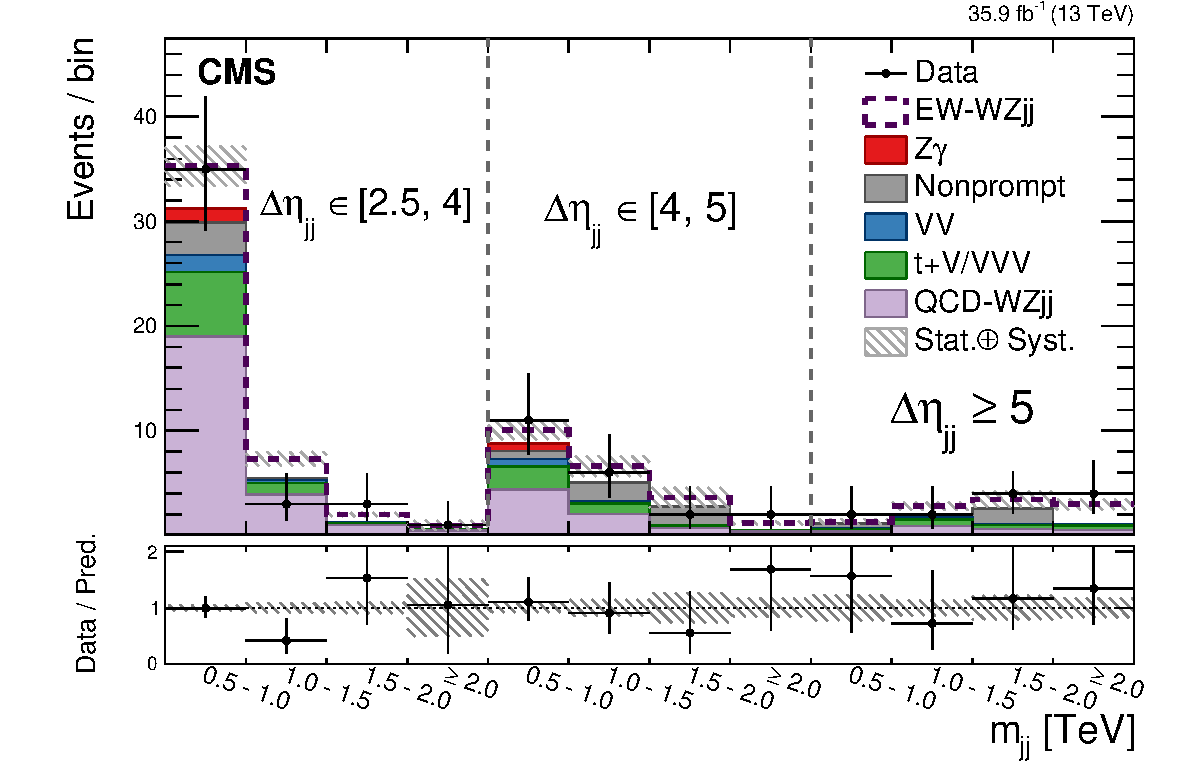
\includegraphics[width=0.7\textwidth]{figures/AnalysisResults/mjj_etajj_unrolled.pdf}
    \caption{
      The one-dimensional representation of the 2D distribution of 
      $\mjj$ and $\left|\etajj\right|$, used for the EW 
      signal extraction. The x axis shows the dijet mass distribution
      in the indicated bins, split into three bins of {\etajj }: {\etajj} $\in [2.5, 4], [4, 5], \ge 5$.
      The dashed line represents the \EWWZ contribution stacked
      on top of the backgrounds, which are shown as filled histograms. 
      The hatched bands represent the total and relative 
      systematic uncertainties on the predicted yields.
      The bottom panel shows the ratio of the number of events measured in data to the total 
      number of expected events. 
      The predicted yields are shown with their best fit normalizations.
    }
  \label{fig:2DfitDistribution}
\end{figure}
\section{New physics searches}

\subsection{Limits on anomalous quartic gauge couplings}

\begin{figure}[htbp]
  \centering
    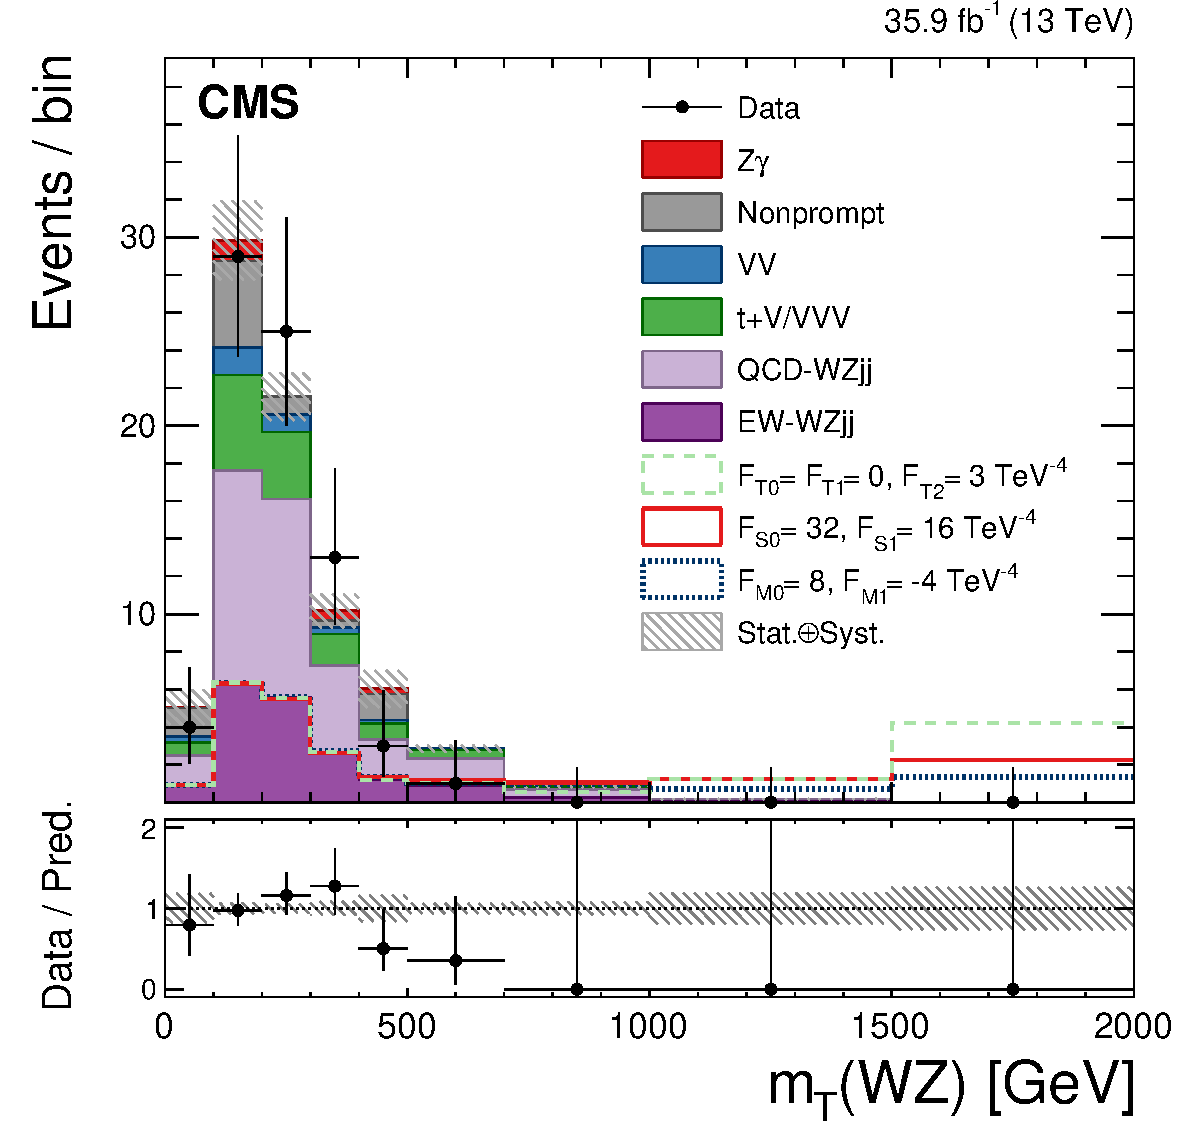
\includegraphics[width=0.5\textwidth]{figures/AnalysisResults/MTWZ_aQGC.pdf}
  \caption{Transverse mass of the \WZ system
      for events satisfying the EW signal selection,
      used to place constraints on the anomalous coupling parameters.
      The \EWWZ contribution, which is treated as background in the fit, is shown as a filled histogram.
      The dashed lines show predictions for several aQGC parameters values, which include the \EWWZ process.
      Normalizations are shown as the best fit values from the background-only fit.
      The last bin also contains all events with transverse mass greater than 2000 GeV.
      Other details as in the caption of Fig.~\ref{fig:VBSPlots}.
      }
 \label{fig:aQGCDistribution}
\end{figure}

\subsection{Limits on charged Higgs boson production}

\begin{figure}[htbp]
  \centering
   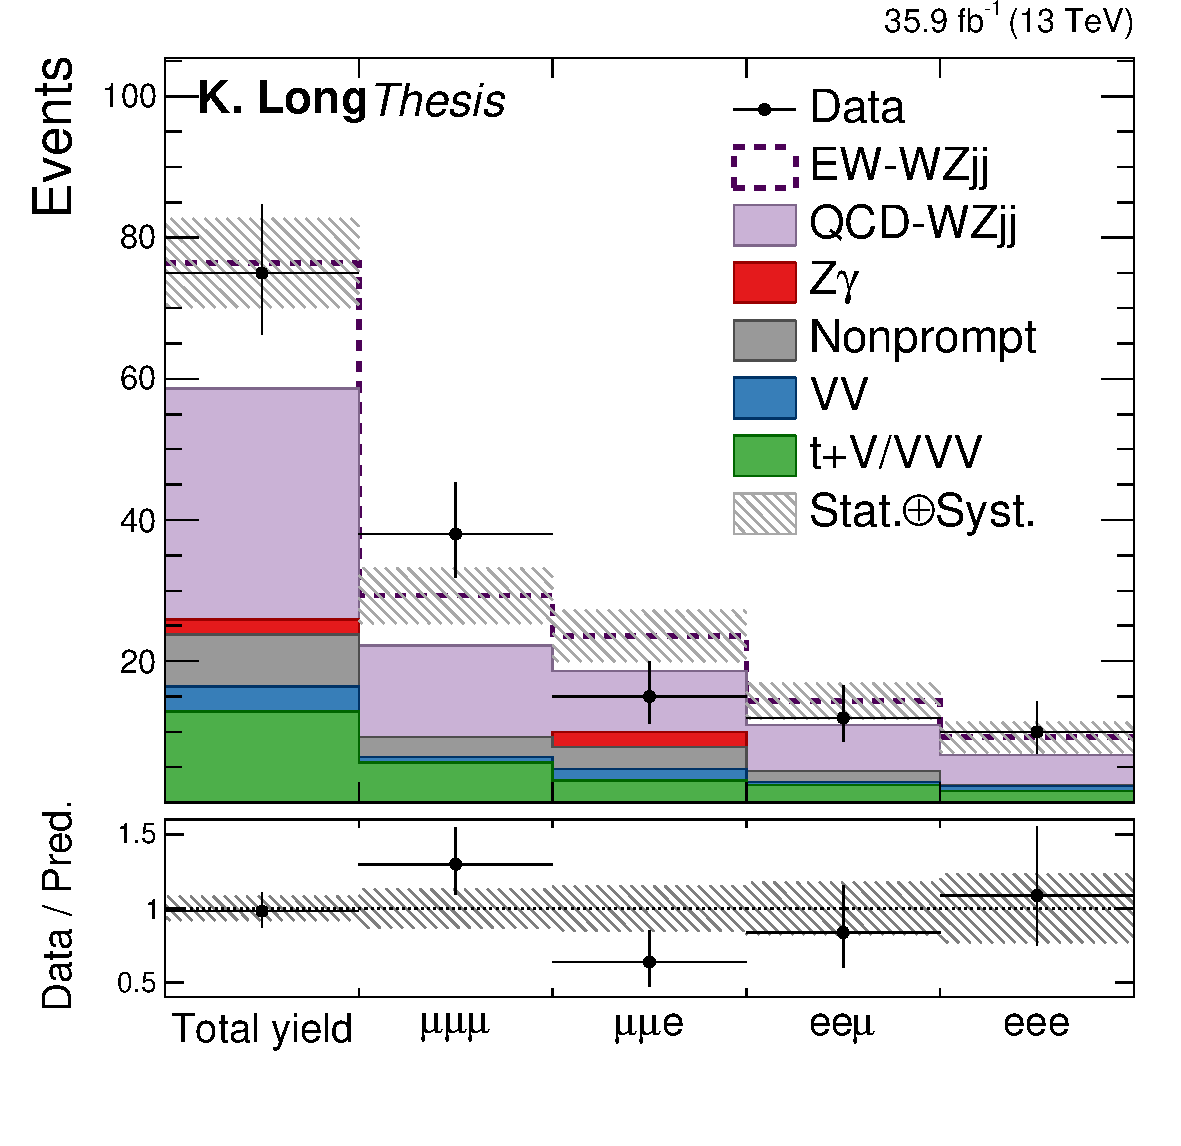
\includegraphics[width=0.7\textwidth]{figures/AnalysisResults/yieldByChannel.pdf}
  \caption{
    Post fit event yields in the charged Higgs boson search region.
          }
 \label{fig:EWSignalYields}
\end{figure}

